\chapter{Materiais utilizados}

\section{Receptor Investigado}

A Tuberculose, causada pela bactéria \emph{Mycobacterium tuberculosis}, é a segunda doença infecciosa que mais causa mortes em todo o mundo. O tratamento com os principais fármacos utilizados atualmente tem duração, em média, de 6 meses e apresenta diversos efeitos colaterais. Muitas vezes o paciente interrompe precocemente o tratamento, propiciando o surgimento de bactérias resistentes aos compostos químicos. Em função disso, o desenvolvimento de novos fármacos ou a melhoria de compostos químicos já existentes é um esforço necessário para controle e combate a Tuberculose.

Dentro deste cenário, o LABIO da PUCRS realiza pesquisas e estudos \emph{in-silico} utilizando como receptor a enzima InhA da \emph{Mycobacterium tuberculosis} e através de experimentos de docagem molecular procura identificar potenciais candidatos à fármaco. A Figura \ref{fig:inha} ilustra a estrutura 3D em formato de fita da proteína InhA.

\begin{figure}[h]
	\center
	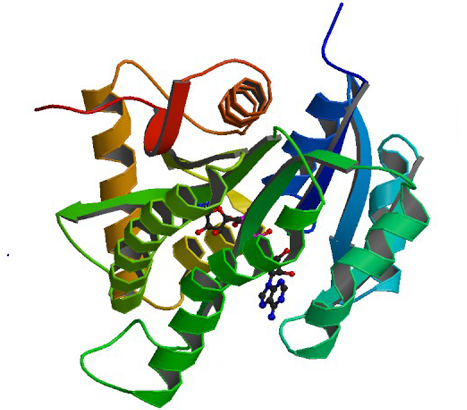
\includegraphics[width=12cm]{images/inha.png}
	\caption{Estrutura 3D em formato de fita da proteína InhA. Imagem obtida em RCSB PDB (www.rcsb.org) do PDB ID 1ENY}
	\label{fig:inha}
\end{figure}

Em sua estrutura, a proteína InhA contém um conjunto de 268 resíduos, que por sua vez são compostos por um total de 4.008 átomos. No PDB (\emph{Protein Data Bank}), a proteína em estudo está identificada pelo código 1ENY.

Conforme descrito em \cite{kar11}, ``A InhA é uma enzima importante no mecanismo de ação da tuberculose pois é responsável pela biossíntese de ácidos graxos, um importante componente da parede celular da micobactéria, e, consequentemente, uma das estruturas essenciais para a sua sobrevivência. Por esse motivo, desperta atenção especial como alvo atraente para o desenvolvimento de novos fármacos para a tuberculose.''

\section{Ligantes Considerados}

O Triclosano (do inglês TCL - \emph{Triclosan}) é um componente químico utilizado para contenção ou prevenção de contaminações bacterianas. É comumente encontrado em produtos domésticos como medicamentos, loções e cremes dentais \cite{TCL}. O TCL está sendo testado como uma alternativa para o desenvolvimento da tuberculose pois age diretamente na inibição do crescimento da bactéria.

De acordo com \cite{GAU08} ``estudos demonstraram que o triclosan também inibe uma enoil-redutase presente em \emph{M. smegmatis} e M. \emph{tuberculosis}. Essa enzima está envolvida com a síntese de ácidos micólicos que são componentes essenciais para a parede celular das  micobactérias e é o principal alvo da INH, um dos mais importantes antimicrobianos utilizados no tratamento da TB.''

A estrutura do TCL consiste em uma pequena molécula composta por um conjunto de 24 átomos. A Figura \ref{fig:tcl} ilustra a estrutura 3D do ligante TCL.

\begin{figure}[h]
	\center
	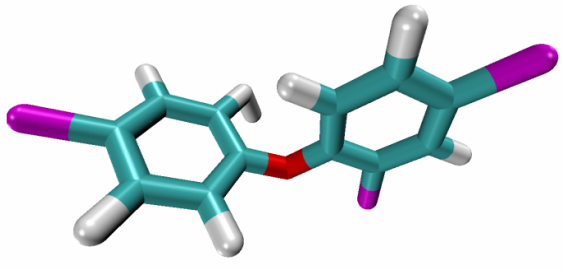
\includegraphics[width=12.5cm]{images/tcl.png}
	\caption{Representação 3D da estrutura do ligante Triclosano \cite{kar11}.}
	\label{fig:tcl}
\end{figure}

Outro ligante empregado nos experimentos de docagem molecular utilizados neste trabalho é o Etionamida (do inglês ETH - \emph{Ethionamide}). O ETH é um antibiótico utilizado no tratamento da tuberculose. É um componente quimico eficaz contra microorganismos do gênero \emph{Mycobacterium}, especialmente as espécies \emph{M. tuberculosis}. 

Conforme descrito em \cite{COH10} ``A ETH se liga covalentemente ao carbono 4 da porção nicotinamida do NADH formando o aduto ETH-NADH, […], este aduto desestabiliza as ligações covalentes que mantêm o NADH em posição no sitio ativo da proteína inibindo a ação da mesma.''

A estrutura do ETH consiste em uma pequena molécula composta por um conjunto de 21 átomos. A Figura \ref{fig:eth} ilustra a estrutura 3D do ligante ETH.

\begin{figure}[h]
	\center
	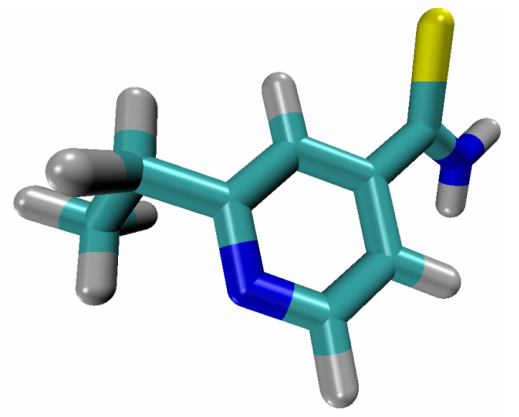
\includegraphics[width=9.5cm]{images/eth.png}
	\caption{Representação 3D da estrutura do ligante Etionamida \cite{kar11}.}
	\label{fig:eth}
\end{figure}

\section{Banco de simulações de docagem}

Primeiramente, os especialistas de domínio do LABIO executaram dois experimentos de docagem molecular, cada um deles envolvendo um ligante diferente. Para o primeiro experimento, foi considerado o TCL como ligante. Já para o segundo, foi utilizado o ligante ETH. Ambos experimentos empregaram a enzima InhA como receptora, e sua flexibilidade foi representada por um conjunto de 3.100 \emph{snapshots} resultantes de simulações por DM. 

Cada ligante foi submetido a 3.100 simulações de docagem, uma para cada conformação do conjunto. Os atributos calculados por estes experimentos foram FEB e RMSD, e após a execução, os dados resultantes dos experimentos foram exportados para um \emph{data set} em formato CSV (\emph{Comma-separated values}).

Neste \emph{data set} os dados estão organizados da seguinte maneira: cada linha representa um dos 3.100 \emph{snapshots} da proteína receptora; nas colunas estão os valores das diferentes posições tridimensionais de cada um dos átomos da proteína e o posicionamento final de cada ligante com seus respectivos valores de FEB e RMSD.

Cada átomo da proteína está representado no \emph{data set} por três colunas, cada uma delas contém respectivamente as coordenadas X, Y e Z de seu posicionamento. As colunas finais apresentam os melhores valores para as métricas FEB e RMSD para cada ligante do experimento. A Tabela \ref{tab:dataset} apresenta a estrutura em que os dados estão organizados no \emph{data set}.

\begin{table}[h]
\caption{Estrutura do \emph{data set} contendo os dados resultantes de experimentos de docagem molecular para os ligantes TCL e ETH.}
\label{tab:dataset}
\resizebox{\textwidth}{!}{%
\begin{tabular}{cllllllll}
\toprule
\textbf{SS}   & \textbf{ALA\_1\_N\_x} & \textbf{ALA\_1\_N\_y} & \textbf{ALA\_1\_N\_z} & \textbf{...} & \textbf{ETHFEB} & \textbf{ETHRMSD} & \textbf{TCLFEB} & \textbf{TCLRMSD} \\ \midrule
\textbf{1}    & 15.834                                     & -20.243                                    & 8.161                                      & ...                               & -8.74                                    & 3.79                                      & -10.52                                   & 5.52                                     \\ 
\textbf{2}    & 15.641                                     & -20.046                                    & 8.011                                      & ...                               & -9.34                                    & 3.86                                      & -9.71                                    & 5.77                                     \\ 
\textbf{3}    & 15.954                                     & -20.459                                    & 7.796                                      & ...                               & -9.38                                    & 3.60                                      & -9.86                                    & 5.45                                     \\ 
\textbf{4}    & 16.321                                     & -20.608                                    & 7.448                                      & ...                               & -9.28                                    & 3.72                                      & -9.23                                    & 5.18                                     \\ 
\textbf{...}  & ...                                        & ...                                        & ...                                        & ...                                         & ...                               & ...                                      & ...                                       & ...                                   \\ 
\textbf{3100} & 18.591                                     & -17.334                                    & 11.449                                     & ...                               & -9.28                                    & 5.28                                      & 1.25                                     & 7.50                                     \\ \bottomrule 
\end{tabular}
}
\end{table}

Relacionando com o processo de ETL, o \emph{data set} recebido representa uma fonte de dados que deve ser utilizada para extração das informações relevantes para a pesquisa. Os dados contidos nele não possuem um tratamento, mas foi possível observar uma padronização de nomenclatura das colunas.
